\documentclass[tikz, crop, border = {2pt 2pt 2pt 2pt}]{standalone}

\usepackage{concmath-otf}
\usetikzlibrary{calc, angles, quotes, patterns}
\usetikzlibrary{decorations.pathreplacing, decorations.pathmorphing, calligraphy}

\begin{document}
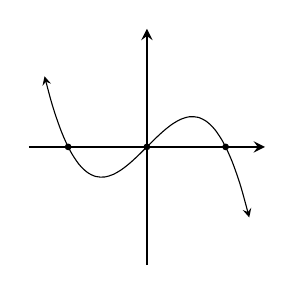
\begin{tikzpicture}
	\draw[-stealth, thick] (-1.5, 0) -- (1.5, 0);
	\draw[-stealth, thick] (0, -1.5) -- (0, 1.5);

	\draw[domain = -1.3:1.3, smooth, stealth-stealth] plot (\x, {- \x^3 + \x});
	\filldraw (0, 0) circle (1pt);
	\filldraw (1, 0) circle (1pt);
	\filldraw (-1, 0) circle (1pt);
\end{tikzpicture}
\end{document}
